%
%% SPDX-License-Identifier: CC-BY-NC-SA-4.0
%%

\documentclass[10pt,a4paper,twoside,american]{article}
\usepackage{geometry}
\geometry{verbose,a4paper,tmargin=2cm,bmargin=2cm,lmargin=2cm,rmargin=2cm}
\usepackage[]{float}
\usepackage[table]{xcolor}
\definecolor{shadecolor}{gray}{0.9}
\usepackage{amsmath}
\usepackage{amssymb}
\usepackage{mathtools}
\usepackage{bm}
\usepackage{natbib}
\usepackage{diagbox}
\usepackage[%%
breaklinks=true,
colorlinks=true,
linkcolor=blue,citecolor=blue,urlcolor=blue,filecolor=blue,
pdffitwindow,
bookmarks=true,
bookmarksopen=true,
bookmarksnumbered=true,
pdftitle={},
pdfauthor={},
pdfsubject={},
pdfkeywords={}
]
{hyperref}
\usepackage{enumitem}
%\usepackage{units}
\usepackage{multirow}

\renewcommand\familydefault{cmss}

\usepackage{cleveref}
\usepackage{setspace}

%%%%%%%%%%%%%%%%%%%%%%%%%%%%%%%%%%%%%%%%%%%%%%%%%%%%%%%%
%% configuration of model-component definitions
\usepackage{amsthm}
\crefformat{definition}{$^\text{#2#1#3}$}
\Crefformat{definition}{$^\text{#2#1#3}$}
%%
\newtheoremstyle{definitionstyle}{2ex}{2ex}{}{0ex}{}{\!}{ }{$^\text{\thmnumber{#2}}$}
\theoremstyle{definitionstyle}
\newtheorem{definition}{}

%%%%%%%%%%%%%%%%%%%%%%%%%%%%%%%%%%%%%%%%%%%%%%%%%%%%%%%%%%%%%%%%%%%%%%%%%%%%%%%%%%%%
%% macros
\newcommand{\diff}{\ensuremath{\text{d}}}
\newcommand{\dtsim}{\Delta t}
\newcommand{\Epop}{\mathcal{E}} %% set (hence caligraphic) of excitatory neurons
\newcommand{\exc}{\text{E}}     %% label for ``excitatory'
\newcommand{\ext}{\text{X}}   %% label for ``external''
\newcommand{\inh}{\text{I}}     %% label for ``inhibitory''
\newcommand{\Ipop}{\mathcal{I}} %% set (hence caligraphic) of inhibitory neurons
\newcommand{\leak}{\text{L}}              %% label for ``external''
\newcommand{\ms}{\,\text{ms}}
\newcommand{\MOhm}{\,\text{M}\Omega}
\newcommand{\mV}{\,\text{mV}}
\newcommand{\nS}{\,\text{nS}}
\newcommand{\pF}{\,\text{pF}}
\newcommand{\pA}{\,\text{pA}}
\newcommand{\RM}{R_\text{m}}
\newcommand{\CM}{C_\text{m}}
\newcommand{\sps}{\,\text{s}^{-1}}
\newcommand{\Stimulus}{\mathcal{S}} %% set (hence caligraphic) of external spike-train generators
\newcommand{\tauM}{\tau_\text{m}}
\newcommand{\tauR}{\tau_\text{ref}}
\newcommand{\tauS}{\tau_\text{s}}
\newcommand{\note}[1]{\textcolor{red}{[\it #1]}}
\newcommand{\drvd}[1]{\textcolor{gray}{#1}} %% font style for derived parameters

%%%%%%%%%%%%%%%%%%%%%%%%%%%%%%%%%%%%%%%%%%%%%%%%%%%%%%%%%%%%%%%%%%%%%%%%%%%%%%%%%%%% 
\begin{document}

\title{Model description:\\ \textbf{Cortical Microcircuit} \citep{Potjans14}}
\author{}
\date{%
  source: \href{https://github.com/INM-6/microcircuit-PD14-model}{https://github.com/INM-6/microcircuit-PD14-model}\\[1ex]
  last update: \today\\
}
\maketitle
\thispagestyle{empty}
%%%%%%%%%%%%%%%%%%%%%%%%%%%%%%%%%%%%%%%%%%%%%%%%%%%%%%%%%%%%%%%%%%%%%%%%%%%%%%%%%%%%
%% disclaimer
\noindent
This document contains a detailed, implementation independent description of the Cortical Microcircuit model, initially developed by \citet{Potjans14}.
It does not contain any information on specific numerical implementations.
%%
%%%%%%%%%%%%%%%%%%%%%%%%%%%%%%%%%%%%%%%%%%%%%%%%%%%%%%%%%%%%%%%%%%%%%%%%%%%%%%%%%%%%

\def\marg{1ex}
\setlength{\parindent}{0pt}

\tableofcontents
\clearpage
%%%%%%%%%%%%%%%%%%%%%%%%%%%%%%%%%%%%%%%%%%%%%%%%%%%%%%%%%%%%%%%%%%%%%%%%%%%%%%%%%%%%
%%%%%%%%%%%%%%%%%%%%%%%%%%%%%%%%%%%%%%%%%%%%%%%%%%%%%%%%%%%%%%%%%%%%%%%%%%%%%%%%%%%%
\section{Model description}
\label{sec:model_description}
%%%%%%%%%%%%%%%%%%%%%%%%%%%%%%%%%%%%%%%%%%%%%%%%%%%%%%%%%%%%%%%%%%%%%%%%%%%%%%%%%%%%
%% model description table: Summary and Populations
%%
\begin{table}[H]
\renewcommand{\arraystretch}{1.2}
%%%%%%%%%%%%%%%%%%%
\begin{tabular}{
  |@{\hspace*{\marg}}p{0.2\textwidth-2.\marg}@{\hspace*{\marg}}
  |@{\hspace*{\marg}}p{0.8\textwidth-2.\marg}@{\hspace*{\marg}}
  |}
  \hline 
  \multicolumn{2}{|>{\color{white}\columncolor{black}}c|}{\textbf{Summary}}\\
  \hline 
  \textbf{Populations} & $8$ cortical populations in $4$ layers ($\text{L2/3}$, $\text{L4}$, $\text{L5}$,
  $\text{L6}$), driven by a thalamic population ($\mathcal{T}$) and cortico-cortical inputs ($\mathcal{C}$)\\
  \hline 
  \textbf{Connectivity} & random, independent, population specific\\
  \hline 
  \textbf{Neuron model} & cortex: leaky integrate-and-fire (LIF); thalamus, cortico-cortical inputs: Poisson point process\\
  \hline 
  \textbf{Synapse model} & exponential postsynaptic currents with static, normally distributed weights and delays\\
  \hline 
  \textbf{Predictions} & population specific spiking activity\\

  \hline
  \multicolumn{2}{|c|}{\centering\parbox{0.95\linewidth}{\centering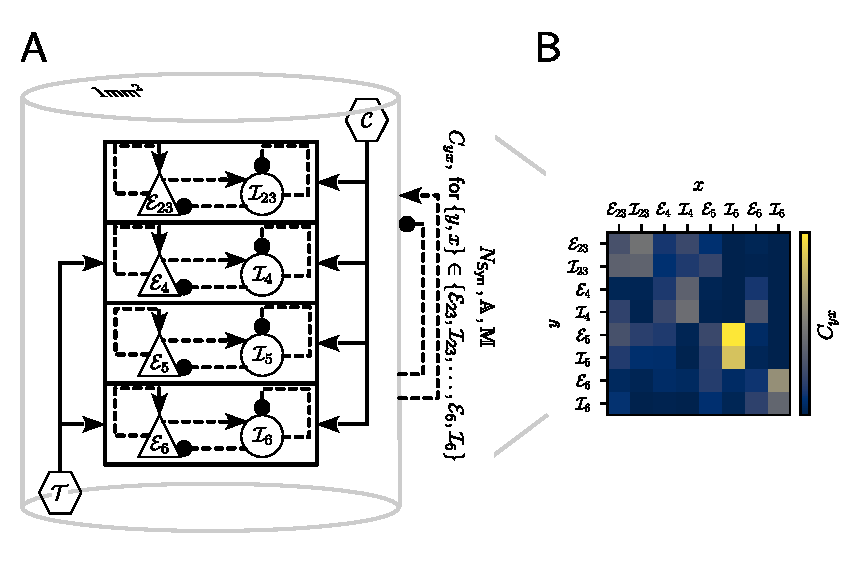
\includegraphics{figures/NetworkSketch_microcircuit-PD14-model.pdf}\\[-5ex] \hfill (see \href{https://doi.org/10.1371/journal.pcbi.1010086.g008}{legend})}}\\
  \hline
\end{tabular}
%%%%%%%%%%%%%%%%%%% 
\begin{tabular}{
  |@{\hspace*{\marg}}p{0.4\textwidth-2.\marg}@{\hspace*{\marg}}
  |@{\hspace*{\marg}}p{0.4\textwidth-2.\marg}@{\hspace*{\marg}}
  |@{\hspace*{\marg}}p{0.2\textwidth-2.\marg}@{\hspace*{\marg}}
  |}
  \hline 
  \multicolumn{3}{|>{\color{white}\columncolor{black}}c|}{\textbf{Populations}}\\
  \hline 
  \textbf{Name} & \textbf{Elements} & \textbf{Size}\\
  \hline
  cortical populations & LIF & $N_{x}$ \\
  $x \in \{\mathcal{E}_{23},\mathcal{E}_{4},\mathcal{E}_{5},\mathcal{E}_{6},\mathcal{I}_{23},\mathcal{I}_{4},\mathcal{I}_{5},\mathcal{I}_{6}\}$ & & \\
  \hline 
  total network $\mathcal{P} = \bigcup_{x} x$ & LIF & $N= \sum_{x} N_{x}$\\
  & & (see remark \ref{remark:network_scaling})\\
  \hline
  cortico-cortical subpopulations $\mathcal{C}_{x}$ & population specific constant currents & $N_{x}$ \\
  \hline
  total population of cortico-cortical inputs & population specific constant currents & $N= \sum_{x} N_{x}$ \\
  $\mathcal{C} = \bigcup_{x} \mathcal{C}_x$ & & \\ 
  \hline 
   thalamic inputs $\mathcal{T}$ & realizations of Poisson point process & $N_{\mathcal{T}}$ \\
  \hline 
\end{tabular}
%%%%%%%%%%%%%%%%%%%
\caption{Description of the network model (continued on next page).}
\label{tab:model_description}
\end{table}
\clearpage
%%%%%%%%%%%%%%%%%%%%%%%%%%%%%%%%%%%%%%%%%%%%%%%%%%%%%%%%%%%%%%%%%%%%%%%%%%%%%%%%%%%%
%% model description table (continued): Connectivity
%%
\addtocounter{table}{-1}
\begin{table}[H]
%%%%%%%%%%%%%%%%%%%
%%%%%%%%%%%%%%%%%%% 
\begin{tabular}{
  |@{\hspace*{\marg}}p{0.2\textwidth-2.\marg}@{\hspace*{\marg}}
  |@{\hspace*{\marg}}p{0.2\textwidth-2.\marg}@{\hspace*{\marg}}
  |@{\hspace*{\marg}}p{0.6\textwidth-2.\marg}@{\hspace*{\marg}}
  |}
  \hline 
  \multicolumn{3}{|>{\color{white}\columncolor{black}}c|}{\textbf{Connectivity}}\\
  \hline
  \textbf{Source} & \textbf{Target} & \textbf{Pattern}\\
  \hline
  $x \in \{\mathcal{E}_{23},\ldots,\mathcal{I}_{6}\}$ & $y \in \{\mathcal{E}_{23},\ldots,\mathcal{I}_{6}\}$ &
                            \vspace{-1ex}                                                                                  
                            \begin{itemize}[topsep=0pt,leftmargin=*]
				    \item random, fixed total number $Q_{yx}$ of connections\cref{def:random_fixed_total_number} (see remark \ref{remark:network_scaling})
                            \item synaptic weights $J_{ij}$ ($\forall{}i\in y, j\in x$)
                            \item spike-transmission delays $d_{ij}$ ($\forall{}i\in y, j\in x$)
                            \end{itemize}\\
  \hline
  $\mathcal{T}$ & $y \in \{\mathcal{E}_{23},\ldots,\mathcal{I}_{6}\}$ &
                            \vspace{-1ex}                                               
                            \begin{itemize}[topsep=0pt,leftmargin=*]
				    \item random, fixed total number $Q_{y\mathcal{T}}$ of connections\cref{def:random_fixed_total_number} 
                            \item synaptic weights $J_{ij}$ ($\forall{}i\in y, j\in \mathcal{T}$)                            \item spike-transmission delays $d_{ij}$ ($\forall{}i\in y, j\in \mathcal{T}$)
                            \end{itemize}\\
  \hline
  $\mathcal{C}_{y}$ & $y \in \{\mathcal{E}_{23},\ldots,\mathcal{I}_{6}\}$ &
                            \vspace{-1ex}                                                   
                            \begin{itemize}[topsep=0pt,leftmargin=*]
				                    \item one-to-one\cref{def:one_to_one}
                            \end{itemize}\\
  \hline
  \multicolumn{3}{|p{0.95\linewidth}|}{%
  %%
  \vspace{-1ex}
  Connectivity patterns:
  \begin{definition}
    \label{def:random_fixed_total_number}
    \emph{random, fixed total number} ($N_\text{Syn}$):
	  This rule establishes a total number of
	  \begin{equation}
		  Q_{yx} = \frac{\text{ln}\left(1-C_{yx}\right)}{\text{ln}\left(1-\left(N_{x}N_{y}\right)^{-1}\right)},
	  \end{equation}
	  connections between a source population $x$ of size $N_x$ and a target population $y$ of size $N_y$.
          $C_{yx}$ denotes the connection probability.
          Sources and targets are randomly and independently drawn from $x$ and $y$ with replacement.
	  Multiple connections between two neurons and self-connections are permitted ($\mathbb{M}$, $\mathbb{A}$).
          %%
  \end{definition}
  \begin{definition}
    \label{def:one_to_one}
    \emph{one-to-one} ($\delta$):
    Each neuron in the source population is connected to one corresponding neuron in the target population (bijection).
  \end{definition}
  \hfill(see ``Network sketch'' above and \citealp{Senk22_e1010086})
  }\\
  \hline
\end{tabular}
%%%%%%%%%%%%%%%%%%%
\caption{Description of the network model (continued).}
\label{tab:model_description_1}
\end{table}
\clearpage
%%%%%%%%%%%%%%%%%%%%%%%%%%%%%%%%%%%%%%%%%%%%%%%%%%%%%%%%%%%%%%%%%%%%%%%%%%%%%%%%%%%%
%% model description table: Neurons
%%
\begin{table}[H]
\renewcommand{\arraystretch}{1.2}
%%%%%%%%%%%%%%%%%%% 
\begin{tabular}{
  |@{\hspace*{\marg}}p{0.2\textwidth-2.\marg}@{\hspace*{\marg}}
  |@{\hspace*{\marg}}p{0.8\textwidth-2.\marg}@{\hspace*{\marg}}
  |}
  \hline 
  \multicolumn{2}{|>{\color{white}\columncolor{black}}c|}{\textbf{Neurons}}\\
  \hline
  \multicolumn{2}{|>{\color{black}\columncolor{lightgray}}c|}{\textbf{Cortical neurons}}\\
  \hline
  \textbf{Type} & leaky integrate-and-fire (LIF)\\
  \hline 
  \textbf{Description} & dynamics of membrane potential $V_{i}(t)$ and spiking activity $s_i(t)$ of neuron $i\in x$ for $x\in\{\mathcal{E}_{23},\ldots,\mathcal{I}_{6}\}$:
                         \begin{itemize}
                         \item emission of $k$th ($k=1,2,\ldots$) spike of neuron $i$ at time $t_{i}^{k}$ if
                           \begin{equation}
                             V_{i}\left(t_{i}^{k}\right)\geq\theta  
                           \end{equation}
                           with spike threshold $\theta$
                         \item reset and refractoriness:
                           \begin{equation}
				   \forall{}k,\ \forall t \in \left[t_{k}^{i},\,t_{k}^{i}+\tauR\right]:\quad V_{i}(t)=V_\text{reset}  
                           \end{equation}
                            with refractory period $\tauR$ and reset potential $V_\text{reset}$
                         \item spike train $\displaystyle s_i(t)=\sum_k \delta(t-t_i^k)$
                         \item subthreshold dynamics of membrane potential $V_{i}(t)$:
                           \begin{equation}
			     \label{eq:membrane_potential}
                             \begin{aligned}
                               &\forall{}k,\ \forall t \notin \left[t_{i}^{k},\,t_{i}^{k}+\tauR\right):\\
                               &\qquad\tauM\frac{\diff{}V_i(t)}{\diff{}t} =
                               \Bigl[E_\text{L}-V_i(t)\Bigr]+\RM I_i(t) + \RM I_{i,\mathcal{C}_y}
                             \end{aligned}
                           \end{equation}
                           with membrane time constant $\tauM$, membrane resistance $\RM$, resting potential $E_\text{L}$, total synaptic input current $I_i(t)$ (see ``Synapses''), and constant background current $I_{i,\mathcal{C}_y}=I_{\mathcal{C}_y}$ for $i\in{}y$ (see ``Cortico-cortical inputs'')
                        \item[] (see App.\,\ref{sec:normal_form} for the normal form of the combined subthreshold neuron-synapse dynamics)
                         \end{itemize}\\
  \hline 
  \multicolumn{2}{|>{\color{black}\columncolor{lightgray}}c|}{\textbf{Thalamic neurons}}\\
  \hline
  \textbf{Type} & Poisson point process \\
  \hline 
  \textbf{Description} &  spike trains $s_{i}(t)$ ($i\in\mathcal{T}$) modeled as independent realizations of Poisson point process with piece-wise constant rate
  \begin{equation}
    \nu_{\mathcal{T}}(t) =
    \begin{cases}
      0 & t<t_\text{start}\\
       \nu_{\mathcal{T}} & t_\text{start} \le t < t_\text{stop}\\
      0 & t\ge{}t_\text{stop}\\
    \end{cases}
  \end{equation}\\
  \hline
  \multicolumn{2}{|>{\color{black}\columncolor{lightgray}}c|}{\textbf{Cortico-cortical inputs}}\\
  \hline
  \textbf{Type} & constant (direct) currents (DC) \\
  \hline 
	\textbf{Description} & population specific constant input current of magnitude
                               \begin{equation}
                                 I_{\mathcal{C}_y} = K_{y\mathcal{C}_y} \cdot \tauS \cdot \bar{I}_{y\mathcal{C}_y} \cdot \nu_{\mathcal{C}_y} 
                                 \quad (\forall y\in\{\mathcal{E}_{23},\ldots,\mathcal{I}_{6}\})\, ,
                               \end{equation}
                               mimicking the mean input resulting from a superposition of $K_{y\mathcal{C}_y}$ spike trains with constant rates $\nu_{\mathcal{C}_y}$, filtered by an exponential kernel with amplitude (weight) $\bar{I}_{y\mathcal{C}_y}$ and time constant $\tauS$ (see remark \ref{remark:cortico_cortical_dc})
  \\
  \hline
  
\end{tabular}
%%%%%%%%%%%%%%%%%%%
\caption{Description of the network model (continued).}
\label{tab:model_description_2}
\end{table}
\clearpage
%%%%%%%%%%%%%%%%%%%%%%%%%%%%%%%%%%%%%%%%%%%%%%%%%%%%%%%%%%%%%%%%%%%%%%%%%%%%%%%%%%%%
%% model description table: Synapses
%%
\begin{table}[H]
\begin{tabular}{
  |@{\hspace*{\marg}}p{0.2\textwidth-2.\marg}@{\hspace*{\marg}}
  |@{\hspace*{\marg}}p{0.8\textwidth-2.\marg}@{\hspace*{\marg}}
  |}
  \hline 
  \multicolumn{2}{|>{\color{white}\columncolor{black}}c|}{
  \textbf{Synapses}
  }\\
  \hline 
  \textbf{Type} & exponential postsynaptic currents with static weights and delays \\
  \hline 
  \textbf{Description} &
  \begin{itemize}
	  %\item total synaptic input current $I_{ij}(t)$ from neuron $j$ to neuron $i$ ($\forall i \in y\in\{\mathcal{E}_{23},\ldots,\mathcal{I}_{6}\}$ and $\forall j \in x\in\{\mathcal{E}_{23},\ldots,\mathcal{I}_{6}, \mathcal{T}, \mathcal{C}\}$):
	\item total synaptic input current $I_i(t)$ to neuron $i$ ($\forall i \in y\in\{\mathcal{E}_{23},\ldots,\mathcal{I}_{6}\}$) is governed by:
		\begin{equation}
			\label{eq:synaptic_current}
			\left(\frac{\diff}{\diff t} + \frac{1}{\tauS}\right) I_{i} (t) = f_{i}(t)
		\end{equation}
		with superposition from all neurons $j \in x,\;\forall x\in\{\mathcal{E}_{23},\ldots,\mathcal{I}_{6}, \mathcal{T}\}$
		\begin{equation}
			f_{i} (t) = \sum_{x} \sum_{j} f_{ij} (t) = \sum_{x} \sum_{j} \hat{I}_{ij} s_{j}(t-d_{ij})
		\end{equation}
                of weighted spike trains with static synaptic weigths $\hat{I}_{ij}$, synaptic time constant $\tauS$, and spike transmission delays $d_{ij}$
        \item[] (see App.\,\ref{sec:normal_form} for the normal form of the combined subthreshold neuron-synapse dynamics)	
	\item solution of \eqref{eq:synaptic_current} for $\displaystyle f_{ij}(t)=\hat{I}_{ij}s_{j}(t)$ and $I_{ij}(t=0)=0$:
		\begin{equation}
			\text{PSC}_{ij}(t)=\hat{I}_{ij} \exp(-t/\tauS)\Theta(t)
		\end{equation}
		with Heaviside function $\Theta(\cdot)$
	\item[$\curvearrowright$] (exponential decaying) posynaptic current triggered by a single presynaptic spike 
	\item solution of \eqref{eq:membrane_potential} for $I_i(t)=\text{PSC}_{ij}(t)$, $V_i(t=0)=0$, and $E_\text{L}=0$:
                           \begin{equation}
                             \text{PSP}_{ij}(t)=
				     \hat{I}_{ij}\RM \frac{\tauS}{\tauS - \tauM}
				     \left(e^{-t/\tauS}-e^{-t/\tauM}\right) \Theta(t) 
                           \end{equation}
                         \item PSC amplitude (synaptic weight):
                           \begin{equation}                          
                             \hat{I}_{ij}
                             =\frac{J_{ij}}{J_\text{unit}(\tauM,\tauS,\RM)}
                           \end{equation}
                           parameterized by PSP amplitude                    
                           $J_{ij}=\text{max}_t\bigl(\text{PSP}_{ij}(t)\bigr)$ 
                         \item[] with unit PSP amplitude (PSP amplitude for $\hat{I}_{ij}=1$):
                           \begin{equation}
                             J_\text{unit}(\tauM,\tauS,\RM)=
				   \RM\frac{\tauS}{\tauS-\tauM} \left( \left[ \frac{\tauM}{\tauS} \right]^{-\tauM/(\tauM - \tauS)} - \left[ \frac{\tauM}{\tauS} \right]^{-\tauS/(\tauM-\tauS)} \right)
                           \end{equation}
                         \item[] and time to PSP maximum:
                           \begin{equation}
                             t_\text{max} =
				   \frac{\tauS\tauM}{\tauM - \tauS} \text{ln}\left(\frac{\tauM}{\tauS}\right)
                           \end{equation}
  \end{itemize}\\
  \hline
\end{tabular}
%%%%%%%%%%%%%%%%%%%
\caption{Description of the network model (continued).}
\label{tab:model_description_3}
\end{table}
\clearpage
%%%%%%%%%%%%%%%%%%%%%%%%%%%%%%%%%%%%%%%%%%%%%%%%%%%%%%%%%%%%%%%%%%%%%%%%%%%%%%%%%%%% 
%% model description table: Synapses (cnt) and Initial conditions
%%
\begin{table}[H]
\begin{tabular}{
  |@{\hspace*{\marg}}p{0.2\textwidth-2.\marg}@{\hspace*{\marg}}
  |@{\hspace*{\marg}}p{0.8\textwidth-2.\marg}@{\hspace*{\marg}}
  |}
  \hline 
  \multicolumn{2}{|>{\color{white}\columncolor{black}}c|}{
	  \textbf{Synapses (continued)}
  }\\
  \hline 
  \textbf{Description} &
  \begin{itemize}
  \item synaptic weights
  \begin{equation}
	  \hat{I}_{ij} = \begin{cases} 
      \text{max}(0,z_{yx}), & j \in x\in\{\mathcal{E}_{23},\mathcal{E}_{4},\mathcal{E}_{5},\mathcal{E}_{6},\mathcal{T}\} \\
      \text{min}(0,z_{yx}), & j \in x\in\{\mathcal{I}_{23},\mathcal{I}_{4},\mathcal{I}_{5},\mathcal{I}_{6}\} \\
      \bar{I}_{yx}, & j \in x=\mathcal{C}_y \\
      0             & \text{if connection $j\to{}i$ does not exist}
      \end{cases}
  \end{equation}
  with
  \begin{equation}
      z_{yx} \sim\mathcal{N}\left\{\bar{I}_{yx},\,\sigma_{\text{s},yx}^2\right\}
  \end{equation}
  drawn from a normal distribution with mean $\bar{I}_{yx}$, variance $\sigma_{\text{s},yx}^2$
  \item[] note: clipping of synaptic weights leads to a deviation of the total number of synapses with non-zero weights from $K_{yx}$ (see ``Connectivity'')
  \item distributed synaptic delays
  \begin{equation}
      d_{ij} = \begin{cases} 
	      \text{max}(d_\text{min},z_{yx}), & \forall i,\ \forall j \in x\in\{\mathcal{E}_{23},\ldots,\mathcal{I}_{6},\mathcal{T}\} \\
      	\bar{d}_{yx}, & \forall i,\ \forall j \in x=\mathcal{C}_y \\
      \end{cases}
  \end{equation}
  with
  \begin{equation}
      z_{yx} \sim\mathcal{N}\left\{\bar{d}_{yx},\,\sigma_{\text{d},yx}^2\right\}
  \end{equation}
  drawn from a normal distribution with mean $\bar{d}_{yx}$, variance $\sigma_{\text{d},yx}^2$, and minimal delay $d_\text{min}$
  \end{itemize}\\
  \hline
\end{tabular}
%%%%%%%%%%%%%%%%%%%
\begin{tabular}{
  |@{\hspace*{\marg}}p{0.2\textwidth-2.\marg}@{\hspace*{\marg}}
  |@{\hspace*{\marg}}p{0.8\textwidth-2.\marg}@{\hspace*{\marg}}
  |}
  \hline
  \multicolumn{2}{|>{\color{white}\columncolor{black}}c|}{
  \textbf{Initial conditions}
  }\\
\hline
\textbf{Type} & random initial membrane potentials and homogeneous initial synaptic currents\\
\hline
  \textbf{Description} &
  \begin{itemize}
  \item membrane potentials
    \begin{equation}
      V_i(t=0)\sim\mathcal{N}(\bar{V}_{0,x},\sigma_{\text{v},x}^2)
    \end{equation}
  randomly and independently drawn from a normal distribution with mean $\bar{V}_{0,x}$ and variance $\sigma^2_{\text{v},x}$ ($\forall i \in x\in\{\mathcal{E}_{23},\ldots,\mathcal{I}_{6}\}$; see remark \ref{remark:initial_conditions})
  \item synaptic currents: $I_{i}(t=0)=0\,\text{pA}$ ($\forall i \in y\in\{\mathcal{E}_{23},\ldots,\mathcal{I}_{6}\}$)
  \end{itemize}\\
  \hline
\end{tabular}
%%%%%%%%%%%%%%%%%%%
\caption{Description of the network model (continued).}
\end{table}
\clearpage
%%%%%%%%%%%%%%%%%%%%%%%%%%%%%%%%%%%%%%%%%%%%%%%%%%%%%%%%%%%%%%%%%%%%%%%%%%%%%%%%%%%%
%%%%%%%%%%%%%%%%%%%%%%%%%%%%%%%%%%%%%%%%%%%%%%%%%%%%%%%%%%%%%%%%%%%%%%%%%%%%%%%%%%%%
\section{Model parameters}
\label{sec:model_parameters}
%%
\renewcommand{\arraystretch}{1.2}
%%
%%%%%%%%%%%%%%%%%%%%%%%%%%%%%%%%%%%%%%%%%%%%%%%%%%%%%%%%%%%%%%%%%%%%%%%%%%%%%%%%%%%% 
%% parameters table
\def\widthA{0.1}
\def\widthB{0.2}
\def\widthC{0.7}
\begin{table}[H]
%%%%%%%%%%%%%%%%%%% 
  \begin{tabular}{|@{\hspace*{\marg}}p{1.0\textwidth-2.\marg}@{\hspace*{\marg}}|}
    \hline
    \multicolumn{1}{|>{\color{black}\columncolor{lightgray}}c|}{\textbf{Network and connectivity}}\\
    \hline
    \multicolumn{1}{|>{\color{black}\columncolor{white}}c|}{\textbf{Population sizes}}\\
    \hline
    \\
    \multicolumn{1}{|c|}{
      \begin{tabular}{|p{6ex}|p{6ex}|p{6ex}|p{6ex}|p{6ex}|p{6ex}|p{6ex}|p{6ex}|p{6ex}|p{6ex}|}
      \hline
      $x$ & $\mathcal{E}_{23}$ & $\mathcal{I}_{23}$ & $\mathcal{E}_{4}$ & $\mathcal{I}_{4}$ & $\mathcal{E}_{5}$ & $\mathcal{I}_{5}$ & $\mathcal{E}_{6}$ & $\mathcal{I}_{6}$ & $\mathcal{T}$\\
      \hline
      $N_{x}$ & $20,683$ & $5,834$ & $21,915$ & $5,479$ & $4,850$ & $1,065$ & $14,395$ & $2,948$ & $902$\\
      \hline
      \end{tabular}
    }\\
    \\
    \hline
    \multicolumn{1}{|>{\color{black}\columncolor{white}}c|}{\textbf{Connection probabilities} $C_{yx}$}\\
    \hline
    \\
    \multicolumn{1}{|c|}{
    \begin{tabular}{|p{6ex}|p{6ex}|p{6ex}|p{6ex}|p{6ex}|p{6ex}|p{6ex}|p{6ex}|p{6ex}|p{6ex}|}
      \hline
      \diagbox[innerwidth=6ex]{$y$}{$x$} & $\mathcal{E}_{23}$ & $\mathcal{I}_{23}$ & $\mathcal{E}_{4}$ & $\mathcal{I}_{4}$ & $\mathcal{E}_{5}$ & $\mathcal{I}_{5}$ & $\mathcal{E}_{6}$ & $\mathcal{I}_{6}$ & $\mathcal{T}$\\
      \hline
      $\mathcal{E}_{23}$ & $0.1009$ & $0.1689$ & $0.0437$ & $0.0818$ & $0.0323$ & $0.0$ & $0.0076$ & $0.0$ & $0.0$\\
      \hline
      $\mathcal{I}_{23}$ & $0.1346$ & $0.1371$ & $0.0316$ & $0.0515$ & $0.0755$ & $0.0$ & $0.0042$ & $0.0$ & $0.0$\\
      \hline
      $\mathcal{E}_{4}$ & $0.0077$ & $0.0059$ & $0.0497$ & $0.1350$ & $0.0067$ & $0.0003$ & $0.0453$ & $0.0$ & $0.0983$\\
      \hline
      $\mathcal{I}_{4}$ & $0.0691$ & $0.0029$ & $0.0794$ & $0.1597$ & $0.0033$ & $0.0$ & $0.1057$ & $0.0$ & $0.0619$\\
      \hline
      $\mathcal{E}_{5}$ & $0.1004$ & $0.0622$ & $0.0505$ & $0.0057$ & $0.0831$ & $0.3726$ & $0.0204$ & $0.0$ & $0.0$\\
      \hline
      $\mathcal{I}_{5}$ & $0.0548$ & $0.0269$ & $0.0257$ & $0.0022$ & $0.0600$ & $0.3158$ & $0.0086$ & $0.0$ & $0.0$\\
      \hline
      $\mathcal{E}_{6}$ & $0.0156$ & $0.0066$ & $0.0211$ & $0.0166$ & $0.0572$ & $0.0197$ & $0.0396$ & $0.2252$ & $0.0512$\\
      \hline
      $\mathcal{I}_{6}$ & $0.0364$ & $0.0010$ & $0.0034$ & $0.0005$ & $0.0277$ & $0.0080$ & $0.0658$ & $0.1443$ & $0.0196$\\
      \hline
    \end{tabular}
    }\\
    \\
    \hline
  \end{tabular}\\
\begin{tabular}{
    |@{\hspace*{\marg}}p{\widthA\textwidth-2.\marg}@{\hspace*{\marg}}
    |@{\hspace*{\marg}}p{\widthB\textwidth-2.\marg}@{\hspace*{\marg}}
    |@{\hspace*{\marg}}p{\widthC\textwidth-2.\marg}@{\hspace*{\marg}}
    |}
  \hline
%%%%%%%%%%%%%%%%%%%%%%%%%%%%%%%%%%%%%%%%%%%%%%%%%%% 
\multicolumn{3}{|>{\color{black}\columncolor{lightgray}}c|}{\textbf{Neuron}}\\
\hline 
\textbf{Name} & \textbf{Value} & \textbf{Description}\\
\hline
$\theta$ & $-50\mV$ & spike threshold \\
\hline
$E_{\text{L}}$ & $-65\mV$ & resting potential \\
\hline
$\tau_{\text{m}}$ & $10\ms$ & membrane time constant \\
\hline
$C_{\text{m}}$ & $250\pF$ & membrane capacitance \\
\hline
\drvd{$\RM$} & \drvd{$\tauM/C_{\text{m}} = 40\MOhm$} & membrane resistance \\
\hline
$V_{\text{reset}}$ & $-65\mV$ & reset potential \\
\hline
$\tau_{\text{ref}}$ & $2\ms$ & absolute refractory period \\
\hline
$\nu_{\mathcal{T}}$ & $120\sps$ & rate of thalamic neurons \\
\hline
$t_{\text{start}}$ & $700\ms$ & start time of thalamic input\\
\hline
$\Delta{t_{\mathcal{T}}}$ & $10\ms$ & duration of thalamic input \\
\hline
\drvd{$t_{\text{stop}}$} & \drvd{$t_{\text{start}}+\Delta{t_{\mathcal{T}}} = 710\ms$} & stop time of thalamic input\\
\hline
$\nu_{\mathcal{C}_y}$ & $8\sps$ & ``rate'' of cortico-cortical inputs ($\forall y\in\{\mathcal{E}_{23}, \dots, \mathcal{I}_{6}\}$)\\
\hline
\drvd{$I_{y,\mathcal{C}_y}$} & \drvd{$\tauS\nu_{\mathcal{C}}\bar{I}_{y,\mathcal{C}_y} = 0.3 \pA$} & amplitude of cortico-cortical DC inputs ($\forall y\in\{\mathcal{E}_{23}, \dots, \mathcal{I}_{6}\}$)\\
\hline
%%%%%%%%%%%%%%%%
  \multicolumn{3}{|>{\color{black}\columncolor{white}}c|}{\textbf{Population specific cortico-cortical in-degrees} $K_{y\mathcal{C}_y}$}\\
    \hline
    \multicolumn{3}{|c|}{}\\
    \multicolumn{3}{|c|}{
      \begin{tabular}{|p{7ex}|p{7ex}|p{7ex}|p{7ex}|p{7ex}|p{7ex}|p{7ex}|p{7ex}|p{7ex}|p{7ex}|}
      \hline
       $\mathcal{C}_{y}$ & $\mathcal{C}_{\mathcal{E}_{23}}$ & $\mathcal{C}_{\mathcal{I}_{23}}$ & $\mathcal{C}_{\mathcal{E}_{4}}$ & $\mathcal{C}_{\mathcal{I}_{4}}$ & $\mathcal{C}_{\mathcal{E}_{5}}$ & $\mathcal{C}_{\mathcal{I}_{5}}$ & $\mathcal{C}_{\mathcal{E}_{6}}$ & $\mathcal{C}_{\mathcal{I}_{6}}$ & $\mathcal{C}_{\mathcal{T}}$\\
      \hline
      $K_{y\mathcal{C}_{y}}$ & $1600$ & $1500$ & $2100$ & $1900$ & $2000$ & $1900$ & $2900$ & $2100$ & $-$\\
      \hline
      \end{tabular}
    }\\
    \multicolumn{3}{|c|}{}\\
    \hline
\end{tabular}
\caption{Model parameters. Parameters derived from other parameters are marked in gray (continued on next page).}
\end{table}
%%%%%%%%%%%%%%%%%%%%%%%%%%%%%%%%%%%%%%%%%%%%%%%%%%%%%%%%%%%%%%%%%%%%%%%%%%%%%%%%%%%% 
%% parameters table (cnt)
\clearpage
\begin{table}[H]
\begin{tabular}{
    |@{\hspace*{\marg}}p{\widthA\textwidth-2.\marg}@{\hspace*{\marg}}
    |@{\hspace*{\marg}}p{\widthB\textwidth-2.\marg}@{\hspace*{\marg}}
    |@{\hspace*{\marg}}p{\widthC\textwidth-2.\marg}@{\hspace*{\marg}}
    |}
\hline
\multicolumn{3}{|>{\color{black}\columncolor{lightgray}}c|}{\textbf{Synapse}}\\
\hline 
\textbf{Name} & \textbf{Value} & \textbf{Description}\\
\hline 
$J$ & $0.15\mV$ & (mean) weight (PSP amplitude) of excitatory synapses\\
\hline
\drvd{$\bar{I}_{yx}$} &  & synaptic weights\\
	& \drvd{$J/J_{\text{unit}}\approx 87.81\pA$} & $\forall x\in\left\{ \mathcal{E}_{23}, \mathcal{E}_{4}, \mathcal{E}_{5}, \mathcal{E}_{6},\mathcal{T}, \mathcal{C}_y\right\}$, $\forall y\in\left\{\mathcal{E}_{23},\mathcal{E}_{4},\mathcal{E}_{5},\mathcal{E}_{6},\mathcal{I}_{23},\mathcal{I}_{4},\mathcal{I}_{5},\mathcal{I}_{6}\right\}$, except for:\\
	& \drvd{$2J/J_{\text{unit}}$} & $\left(x,y\right)=\left(\mathcal{E}_{23}, \mathcal{E}_{4}\right)$\\
	& \drvd{$-4J/J_{\text{unit}}$} & $\forall x\in\left\{ \mathcal{I}_{23}, \mathcal{I}_{4}, \mathcal{I}_{5}, \mathcal{I}_{6}\right\}$,  $\forall y\in\left\{\mathcal{E}_{23},\mathcal{E}_{4},\mathcal{E}_{5},\mathcal{E}_{6},\mathcal{I}_{23},\mathcal{I}_{4},\mathcal{I}_{5},\mathcal{I}_{6}\right\}$\\
\hline
$\sigma_{\text{s},yx}$ & $0.1\cdot \bar{I}_{yx}$ & standard deviation of weight distribution\\
\hline
$\tau_{\text{s}}$ & $0.5\ms$ &  synaptic time constant \\
\hline
$\bar{d}_{yx}$ &  & mean spike transmission delays\\
              & $1.5\ms$ & $x\in\left\{ \mathcal{E}_{23}, \mathcal{E}_{4}, \mathcal{E}_{5}, \mathcal{E}_{6},\mathcal{T},\mathcal{C}_y\right\} $,
$y\in\left\{\mathcal{E}_{23},\mathcal{E}_{4},\mathcal{E}_{5},\mathcal{E}_{6},\mathcal{I}_{23},\mathcal{I}_{4},\mathcal{I}_{5},\mathcal{I}_{6}\right\}$
  \\
 & $0.75\ms$ & $x\in\left\{ \mathcal{I}_{23}, \mathcal{I}_{4}, \mathcal{I}_{5}, \mathcal{I}_{6}\right\}$, 
$y\in\left\{\mathcal{E}_{23},\mathcal{E}_{4},\mathcal{E}_{5},\mathcal{E}_{6},\mathcal{I}_{23},\mathcal{I}_{4},\mathcal{I}_{5},\mathcal{I}_{6}\right\}$ \\
 \hline
  $\sigma_{\text{d},yx}$ & $0.5\cdot\bar{d}_{yx}$ & standard deviation of spike transmission delays\\
  \hline
  $d_\text{min}$      & $0.1\ms$      & minimal spike transmission delay\\ 
\hline
%%%%%%%%%%%%%%%%%%%%%%%%%%%%%%%%%%%%%%%%%%%%%%%%%%%
\multicolumn{3}{|>{\color{black}\columncolor{lightgray}}c|}{\textbf{Initial conditions}}\\
\hline
\multicolumn{3}{|>{\color{black}\columncolor{white}}c|}{\textbf{Population specific mean and standard deviation of initial membrane-potential distributions}}\\
\hline
\multicolumn{3}{|c|}{}\\
\multicolumn{3}{|c|}{
\begin{tabular}{|p{14ex}|>{\raggedleft}p{7ex}|>{\raggedleft}p{7ex}|>{\raggedleft}p{7ex}|>{\raggedleft}p{7ex}|>{\raggedleft}p{7ex}|>{\raggedleft}p{7ex}|>{\raggedleft}p{7ex}|>{\raggedleft\arraybackslash}p{7ex}|}
	\hline
	population $x$ & $\mathcal{E}_{23}$ & $\mathcal{I}_{23}$ & $\mathcal{E}_{4}$ & $\mathcal{I}_{4}$ & $\mathcal{E}_{5}$ & $\mathcal{I}_{5}$ & $\mathcal{E}_{6}$ & $\mathcal{I}_{6}$\\
        \hline
	\vspace{-1ex} $\bar{V}_{0, x}$ ($\mV$) & \vspace{-1ex} $-68.28$ & \vspace{-1ex} $-63.16$ & \vspace{-1ex} $-63.33$ & \vspace{-1ex} $-63.45$ & \vspace{-1ex} $-63.11$ & \vspace{-1ex} $-61.66$ & \vspace{-1ex} $-66.72$ & \vspace{-1ex} $-61.45$\\
        \hline
	\vspace{-1ex} $\sigma_{\text{v}, x}$ ($\mV$) & \vspace{-1ex} $5.36$ & \vspace{-1ex} $4.57$ & \vspace{-1ex} $4.74$ & \vspace{-1ex} $4.94$ & \vspace{-1ex} $4.94$ & \vspace{-1ex} $4.55$ & \vspace{-1ex} $5.46$ & \vspace{-1ex} $4.48$\\
        \hline
\end{tabular}
}\\
\multicolumn{3}{|c|}{}\\
\hline
\end{tabular}
\caption{Model parameters. Parameters derived from other parameters are marked in gray (continued).}
\end{table}
%%%%%%%%%%%%%%%%%%%%%%%%%%%%%%%%%%%%%%%%%%%%%%%%%%%%%%%%%%%%%%%%%%%%%%%%%%%%%%%%%%%%%
%%%%%%%%%%%%%%%%%%%%%%%%%%%%%%%%%%%%%%%%%%%%%%%%%%%%%%%%%%%%%%%%%%%%%%%%%%%%%%%%%%%%%
\clearpage
\appendix
\section{Single-neuron dynamics in normal form (subthreshold)}
\label{sec:normal_form}
\begin{itemize}
\item linear, inhomogeneous dynamics of synaptic input currents and (subthreshold) membrane potential for neuron $i \in y\in\{\mathcal{E}_{23},\ldots,\mathcal{I}_{6}\}$ (cf.~eqs.\,\eqref{eq:membrane_potential} and \eqref{eq:synaptic_current}):
  \begin{equation}
    \label{eq:1st_order_ode}
    \begin{aligned}
      \dot{I}_{i} + \frac{1}{\tauS} I_{i} &= f_{i}(t)\\
      \dot{V}_{i} + \frac{1}{\tauM} \Bigl[ V_{i}-E_\text{L}\Bigr] - \frac{\RM}{\tauM} I_{i} &= 0
    \end{aligned}
  \end{equation}
  with
  \begin{equation}
	  f_{i}(t)=\sum_{x}\sum_{j\in x} \hat{I}_{ij} s_{j}(t-d_{ij})
    \qquad(x\in\{\mathcal{E}_{23},\ldots,\mathcal{I}_{6}, \mathcal{T}, \mathcal{C}\})
  \end{equation}

\item rescale membrane potential $v_i(t) = V_i(t)-E_\text{L}$ and total
  current $\displaystyle{}x_{i}(t) = \frac{\RM}{\tauM}I_{i}(t)$:
  \begin{equation}
    \label{eq:1st_order_ode_rescaled}
    \begin{aligned}
      \dot{x}_{i} + \frac{1}{\tauS} x_{i} &= \frac{\RM}{\tauM} f_{i}(t)\\
      \dot{v}_{i} + \frac{1}{\tauM} v_{i} -  x_{i}  &= 0
    \end{aligned}
  \end{equation} 
\item normal form of neuron-$i$ dynamics \eqref{eq:1st_order_ode_rescaled}:
  \begin{equation}
    \label{eq:normal_form}
    \frac{\diff}{\diff t} \bm{y}_i = \bm{A} \bm{y}_i + \bm{f}_i(t)
  \end{equation}
  with $D=2$ dimensional state vector
  \begin{equation}
    \label{eq:normal_form_state_vector}    
    \bm{y}_i(t) = 
    \begin{pmatrix}
      x_{i}(t)   \,,\,
      v_{i}(t)       
    \end{pmatrix}^\text{T},
  \end{equation}
  with constant $(D\times{}D)$ matrix
  \begin{equation}
    \label{eq:normal_form_coupling_matrix}    
    \bm{A} = 
    \begin{bmatrix}
      -1/\tauS & 0\\
      1        & -1/\tauM  
    \end{bmatrix},	   
  \end{equation}
  and inhomogeneity vector
  \begin{equation}
    \label{eq:normal_form_inhomogeneity}        
    \bm{f}_i(t) = 
    \begin{pmatrix}\displaystyle
      \frac{\RM}{\tauM} f_{i}(t)     \,,\,
      0               
    \end{pmatrix}^\text{T}
  \end{equation}
  \citep[see Sec.\,3.2.2 in][]{Rotter99_381}
\item see App.\,\ref{sec:exact_integration} for an efficient, exact integration scheme of \eqref{eq:normal_form}
\item back-transform to physical quantities:
  \begin{equation}
    \begin{aligned}
      V_i(t)      & = v_i(t)+E_\text{L}\\
      I_{i}(t) & = \frac{\tauM}{\RM}x_{i}(t)
    \end{aligned}
  \end{equation}
\end{itemize}
%%%%%%%%%%%%%%%%%%%%%%%%%%%%%%%%%%%%%%%%%%%%%%%%%%%%%%%%%%%%%%%%%%%%%%%%%%%%%%%%%%%% 
\section{Exact integration of  single-neuron dynamics (subthreshold)}
\label{sec:exact_integration}

\begin{itemize}
\item exact integration of \eqref{eq:normal_form} for spikes arriving at the target neuron $i$ on a time grid
  \mbox{$\mathcal{T}_\Delta= \{t_k=k\Delta{}|k\in\mathbb{N},\Delta\in\mathbb{R}^+\}$}, i.e.,
  for spike trains \mbox{$s_j(t) = \sum_l\delta(t-t_j^l)$} with $t_j^l\in\mathcal{T}_\Delta$ \citep{Rotter99_381}:
  \begin{equation}
    \label{eq:exact_integration}
    \bm{y}_i(t_{k+1}) = \bm{P}\bm{y}_i(t_k) + \bm{f}_i(t_{k+1})
  \end{equation}
  with $(D\times{}D)$ propagator matrix (matrix exponential)
  \begin{equation}
    \label{eq:matrix_exponential}
    \bm{P} = e^{\bm{A}\Delta}
  \end{equation}
  with components 
  \begin{equation}
    %\def\cnstrntwdth{0.5\linewidth}
    %\def\vspc{3ex}
	\bm{P} =
	\begin{bmatrix}
      		e^{-\Delta/\tauS} 					     & 0\\
		\frac{e^{-\Delta/\tauM}-e^{-\Delta/\tauS}}{1/\tauS-1/\tauM}  & e^{-\Delta/\tauM}
    	\end{bmatrix}
  \end{equation}
  \citep[see Sec.\,3.2.2 in][]{Rotter99_381}
\end{itemize}
%%
%%%%%%%%%%%%%%%%%%%%%%%%%%%%%%%%%%%%%%%%%%%%%%%%%%%%%%%%%%%%%%%%%%%%%%%%%%%%%%%%%%%%
%%%%%%%%%%%%%%%%%%%%%%%%%%%%%%%%%%%%%%%%%%%%%%%%%%%%%%%%%%%%%%%%%%%%%%%%%%%%%%%%%%%%
\section{Remarks}
\label{sec:remarks}
%%
\begin{enumerate}
%%%
%%%%%%%%%%%%%%%%%%%%%%%%%%%%%%%%%%%%%%% 
\item \label{remark:network_scaling}
  In the PyNEST implementation of the model provided \href{https://github.com/INM-6/microcircuit-PD14-model}{here}, the model size can be configured by the parameters \texttt{N\_scaling} and \texttt{K\_scaling}, which scale the number of neurons in the network and the number of synapses per neuron (in-degree), respectively. 
  The original (default) full-scale model corresponds to \texttt{N\_scaling=1} and \texttt{K\_scaling=1}.
  Downscaling the model enables running it in the presence of limited computing resources (e.g., on a laptop).
  The scaling of the synapse number affects both the connections within the local network and the external (cortico-cortical) inputs.
  %% 
  Without any compensation, changing the number of synapses would change the statistics of the total input current
  \begin{equation}
    \label{eq:total_synaptic_input_current}
    I_i(t)=\sum_{x\in\{\mathcal{E}_{23},\ldots,\mathcal{I}_{6}\}} \sum_{j\in{}x} (s_j* \text{PSC}_{ij})(t-d_{ij}) + I_{i,\mathcal{C}}
  \end{equation}
  for each postsynaptic neuron $i$ in population $y\in\{\mathcal{E}_{23},\ldots,\mathcal{I}_{6}\}$, and hence the firing statistics.
  In the PyNEST implementation provided \href{https://github.com/INM-6/microcircuit-PD14-model}{here}, this change in the activity statistics is suppressed by rescaling the average synaptic weights $\bar{I}_{yx}$ and injecting an additional constant input current into each neuron.
  In the following, we outline this compensation procedure.
  %%
  \par  
  Under the assumption that the spike trains $s_j(t)$ can be described by stationary Poisson point processes with rates $\nu_j$, the mean and the variance of the total synaptic input current \cref{eq:total_synaptic_input_current} read\footnote{Here, we have absorbed the constant cortico-cortical input current $I_{i,\mathcal{C}}$ into the sum across all presynaptic sources.}
  \begin{equation}
    \label{eq:mean_and_variances_synaptic_input}
      \mu_i      =             \tauS \sum_{x\in\{\mathcal{E}_{23},\ldots,\mathcal{I}_{6},\mathcal{C}_y\}} \sum_j \hat{I}_{ij}   \nu_j 
      \quad\text{and}\quad
      \sigma_i^2 = \frac{1}{2} \tauS \sum_x \sum_j \hat{I}_{ij}^2 \nu_j  .
  \end{equation}
  If we further assume that the variance $\sigma_{\text{s},yx}^2$ of the synaptic weight distribution can be neglected, the population averaged mean and variance are approximated by
  \begin{equation}
    \label{eq:mean_and_variances_synaptic_input_pop_av}
    \mu_y      =\langle\mu_i\rangle_{i\in{}y}       = \tauS            \sum_x K_{yx}  \bar{I}_{yx}   \nu_x 
    \quad\text{and}\quad
    \sigma_y^2 = \langle\sigma_i^2\rangle_{i\in{}y}  = \frac{1}{2}\tauS \sum_x K_{yx} \bar{I}_{yx}^2 \nu_x  .
  \end{equation}
  Here, $K_{yx}$ refers to the average number of inputs a neuron in population $y$ receives from the presynaptic population $x$, and $\nu_x$ to the population averaged firing rate of neurons in population $x$.
  Without further compensation, scaling the in-degrees $K_{yx}^*=fK_{yx}$ by some factor $f$ would evidently change  $\mu_y$ and $\sigma_y^2$.
  However, if we rescale the synaptic weights according to
  \begin{equation}
    \bar{I}_{yx}^*=\frac{\bar{I}_{yx}}{\sqrt{f}},
  \end{equation}
  the variance of the total input current is remains unchanged:
  \begin{equation}
    (\sigma_y^*)^2
    = \frac{1}{2}\tauS \sum_x K_{yx}^* \bar{I}_{yx}^{*,2} \nu_x
    = \frac{1}{2}\tauS \sum_x fK_{yx} \left(\frac{\bar{I}_{yx}^*}{\sqrt{f}}\right)^2 \nu_x
    = \sigma_y^2.
  \end{equation}
  If we furthermore inject an additional constant input current with amplitude
  \begin{equation}
   \Delta\mu_y = \left(1-\sqrt{f}\right)  \mu_y 
  \end{equation}
  into all neurons in population $y$, we simultaneously preserve the mean of the total input current:
  \begin{equation}
    \mu_y^*
    = \tauS \sum_x K_{yx}^*  \bar{I}_{yx}^*   \nu_x + \Delta\mu_y
    = \tauS \sum_x f K_{yx}  \frac{\bar{I}_{yx}}{\sqrt{f}}   \nu_x +  \Delta\mu_y
    = \sqrt{f} \mu_y  +  \left(1-\sqrt{f}\right)  \mu_y
    =  \mu_y.
  \end{equation}
  (see remark \ref{remark:dc_scaling_constraints}).
  For more details and other scaling methods, see \citep{vanAlbada15}.
%%%
%%%%%%%%%%%%%%%%%%%%%%%%%%%%%%%%%%%%%%% 
\item \label{remark:cortico_cortical_dc}
  In the original model of \citet{Potjans14}, the cortico-cortical inputs to neurons in population $y$ are modeled as $K_{y\mathcal{C}_{y}}$ independent realizations $s_j(t)$ ($j\in\mathcal{C}_y,\ y\in \{\mathcal{E}_{23},\ldots,\mathcal{I}_{6}\}$) of a Poisson point process with constant rate $\nu_{\mathcal{C}_y}$, filtered by an exponential kernel $\text{PSC}(t)$ with time constant $\tauS$ and amplitude $\bar{I}_{y\mathcal{C}_y}$.   
  In the implementation provided \href{https://github.com/INM-6/microcircuit-PD14-model}{here}, these Poissonian inputs are replaced by constant external currents (DC).
  DC inputs are computationally less expensive, exactly reproducible, and lead to similar network activity statistics.
  When replacing cortico-cortical input spikes $s_j(t)$ by DC inputs, the current implementation preserves the mean input current
  \begin{equation}
    I_{\mathcal{C}_y}
    = \left\langle \sum_{j=1}^{K_{y\mathcal{C}_y}} \left(s_j*\text{PSC}\right)(t) \right\rangle
    = K_{y\mathcal{C}_y} \cdot \tauS \cdot \bar{I}_{y\mathcal{C}_y} \cdot \nu_{\mathcal{C}_y} .
  \end{equation}
%%%
%%%%%%%%%%%%%%%%%%%%%%%%%%%%%%%%%%%%%%%   
\item \label{remark:dc_scaling_constraints}
  In the scaled version of the model (see remark \ref{remark:network_scaling}), the neurons receive --in addition to the cortico-cortical inputs-- an additional constant input current of magnitude $\Delta\mu_y = ( 1 - \sqrt{f}) \mu_y$ (see remark \ref{remark:network_scaling}).
  The total DC input current injected into neurons of population $y$ is hence given by
  \begin{equation}
    \label{eq:dc_magnitude_rescaled}
    \begin{aligned}
    I_{\text{DC},y}
    & = I_{y\mathcal{C}_y}^* + \left( 1 - \sqrt{f} \right) \mu_y\\
    & = \sqrt{f} I_{y\mathcal{C}_y} + \left( 1 - \sqrt{f} \right) \left( \mu_{y,\text{loc}} + I_{y\mathcal{C}_y}\right) \\
    & = I_{y\mathcal{C}_y} + \left( 1 - \sqrt{f} \right) \mu_{y,\text{loc}}
    ,      
    \end{aligned}
  \end{equation}
  where $I_{y\mathcal{C}_y}^* = \tauS \cdot fK_{y\mathcal{C}_y} \cdot \bar{I}_{y\mathcal{C}_y}/\sqrt{f} = \sqrt{f} I_{y\mathcal{C}_y}$ denotes the rescaled cortico-cortical input current, and  $\mu_{y,\text{loc}}=\mu_y - I_{y\mathcal{C}_y}$ the mean input current resulting from synaptic inputs from the local network.
  In the absence of any initial spikes, the neurons in the network can generate spikes only if $I_{\text{DC},y}$ exceeds the rheobase current
  \begin{equation}
    \label{eq:rheobase_current}
     I_{\text{rh},y} = \frac{\theta - E_{\text{L}}}{\RM} ,
  \end{equation}
  at least for some of the populations $y$.
  To ensure that population $y$ of the scaled network becomes is activated by the external inputs, the scaling factor $f$ must fulfill
  \begin{equation}
    \label{eq:scaling_factor_constraint}
      I_{y\mathcal{C}_y} + \left( 1 - \sqrt{f} \right) \mu_{y,\text{loc}} \geq I_{\text{rh},y} 
      \quad\Leftrightarrow\quad
      f
      \begin{cases} 
        \ge f_y^* & \text{if}\ \mu_{y,\text{loc}} < 0 \\
        \le f_y^* & \text{if}\ \mu_{y,\text{loc}} > 0 \\
      \end{cases},
  \end{equation}
  with the critical scaling factor
  \begin{equation}
    \label{eq:critical_scaling_factor}
    f_y^* = \left(1 - \frac{I_{\text{rh},y} - I_{y\mathcal{C}_y}}{\mu_{y,\text{loc}}}\right)^2 .
  \end{equation}
  Typically, the mean of the local input current is negative, $\mu_{y,\text{loc}}<0$, due to the dominant inhibitory feedback in balanced networks.
  In this case, the critical scaling factor $f_y^*$ defines a lower bound for $f$.
  If the network is downscaled too much such that $f<f_y^*$ for some population $y$, this population can only be activated by other populations $y'$ where $f>f_{y'}^*$.
%%%
%%%%%%%%%%%%%%%%%%%%%%%%%%%%%%%%%%%%%%%   
\item \label{remark:initial_conditions} The original model of \citet{Potjans14} uses population \emph{unspecific} normal distributions of initial membrane potentials.
By default, the current implementation uses population \emph{specific} initial membrane potential distributions instead to speed up convergence to the stationary state.
In the reference implementation provided \href{https://github.com/INM-6/microcircuit-PD14-model}{here}, the type of initial conditions can be set by the parameter \texttt{V0\_type} (\texttt{"optimized"} [default] or \texttt{"original"}).
In \citep{Senk25_arxiv}, the population specific initial conditions are refered to as \emph{amended} initial conditions.
  %%% 
\end{enumerate}

%%%%%%%%%%%%%%%%%%%%%%%%%%%%%%%%%%%%%%%%%%%%%%%%%%%%%%%%%%%%%%%%%%%%%%%%%%%%%%%%%%%% 
%% references
\clearpage
\begin{thebibliography}{}

\bibitem[Potjans et al., 2014]{Potjans14}
  Potjans, T. C., Diesmann, M. (2014).
  \newblock The cell-type specific cortical microcircuit: relating structure and activity in a full-scale spiking network model. 
  \newblock Cerebral cortex (New York, N.Y. : 1991), 24(3), 785–806.
  \newblock \url{https://doi.org/10.1093/cercor/bhs358}

\bibitem[Rotter \& Diesmann, 1999]{Rotter99_381}
  Rotter, S., and Diesmann, M.~(1999).
  \newblock Exact digital simulation of time-invariant linear systems with applications to neural modeling.
  \newblock {\em Biological Cybernetics}, 81:381--402.

\bibitem[Senk et al., 2022]{Senk22_e1010086}
  Senk, J., Kriener, B., Djurfeldt, M., Voges, N., Jiang, H.-J., Sch\"uttler, L., Gramelsberger, G., Diesmann, M., Plesser, H.E., van Albada, S.J.~(2022).
  \newblock Connectivity concepts in neuronal network modeling.
  \newblock {\em PLoS Computational Biology}, 18(9):e1010086.

  \bibitem[Senk et al., 2025]{Senk25_arxiv}
  Senk, J., Kurth, A., Furber, S., Gemmeke, T., Golosio, B., Heittmann, A., Knight, J. C., M\"uller, E., Noll, T., Nowotny, T., Peraza Coppola, G., Peres, L., Rhodes, O., Rowley, A., Schemmel, J., Stadtmann, T., Tetzlaff, T., Tiddia, G., van Albada, S. J., Villamar, J., \& Diesmann, M. (2025). 
  \newblock Constructive community race: full-density spiking neural network model drives neuromorphic computing.
  \newblock arXiv:2505.21185.

\bibitem[van Albada et al., 2015]{vanAlbada15}
van Albada, S. J., Helias, M., Diesmann, M. (2015).
\newblock Scalability of Asynchronous Networks Is Limited by One-To-One Mapping between Effective Connectivity and Correlations.
\newblock {\em PLoS Computational Biology}, 11(9):e1004490.
\newblock \url{https://doi.org/10.1371/journal.pcbi.1004490}

\end{thebibliography}

\end{document}
%%% Local Variables:
%%% mode: latex
%%% TeX-master: t
%%% End:
